%\setchapterimage{Fond_CIN.png}
\setchapterpreamble[u]{\margintoc}

\chapter{Génie électrique en tension alternative}


%\marginnote[4cm]{
%\UPSTIcompetence[2]{B2-10}
%}

%\marginnote[6cm]{\textbf{Emilien Durif}, \textit{Approche énergétique}, Lycée La Martinière Monplaisir, Lyon.}

\section{Signaux périodiques}

\subsection{Caractéristique des signaux périodiques}

\begin{marginfigure}
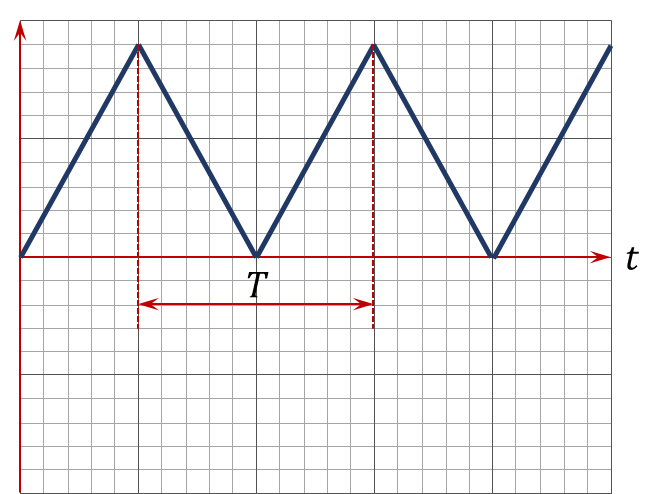
\includegraphics[width=\linewidth]{fig_01}
\caption{Signal périodique \label{fig:ge:cours:01}}
\end{marginfigure}

\begin{defi}[Signal périodique]
Un signal $s(t)$ est dit périodique de période $T$ si $\forall t$, $s(t)=s(t+T)$.
\end{defi}

\begin{defi}[Caractéristiques]
On peut définir : 
\begin{itemize}
\item la fréquence du signal, en Hertz \si{Hz}, $f=\dfrac{1}{T}$;
\item la pulsation, pour un régime sinusoïdal, en \si{rad.s^{-1}} :  $\omega = 2\pi f$;
\item la valeur maximale (ou de crête). 
\end{itemize}
\end{defi}

\subsection{Valeur moyenne}
\begin{marginfigure}
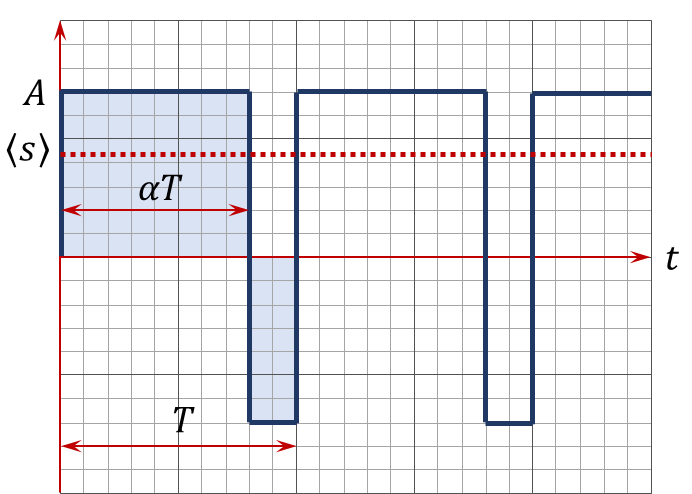
\includegraphics[width=\linewidth]{fig_02}
\caption{Valeur moyenne\label{fig:ge:cours:02}}
\end{marginfigure}


\begin{marginfigure}
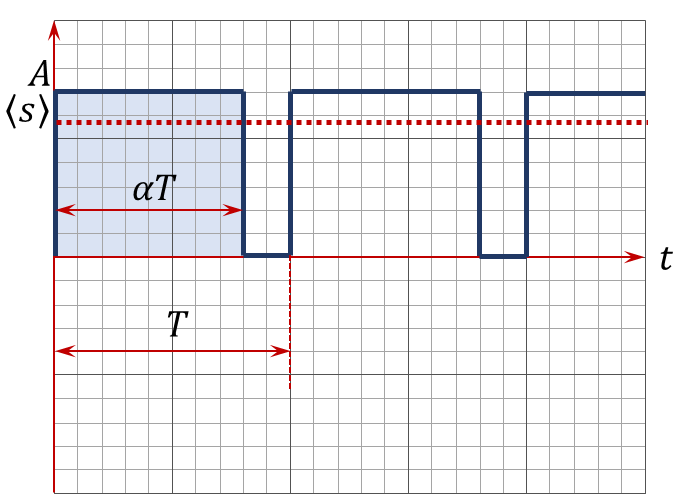
\includegraphics[width=\linewidth]{fig_03}
\caption{Valeur moyenne\label{fig:ge:cours:03}}
\end{marginfigure}

\begin{defi}[Valeur moyenne]
Valeur de la grandeur continue qui créerait la même aire qu'un signal périodique sur une période $T$.
On a alors : 
$$\langle s \rangle = \dfrac{1}{T} \int\limits_{t_0}^{t_0+T} s(t)\; \dd t.$$
\end{defi}

\begin{prop}
Si $s(t) = s_1(t)+s_2(t)$ alors  $\langle s \rangle = \langle s_1 \rangle+\langle s_2 \rangle$.
\end{prop}

La valeur moyenne est celle mesurée par un multimètre en position \textbf{DC} ou \textbf{=}.

Le courant moyen d'un courant périodique serait équivalant au courant continu qui tranporterait la même quantité d'électricité que celle tranportée durant une période.

\subsection{Valeur efficace}
\begin{defi}[Valeur efficace]
La valeur efficace $S$ ou $\indice{S}{eff}$ du signal $s(t)$ est donnée par  
$$\indice{S}{eff} = \sqrt{\dfrac{1}{T} \int\limits_{t_0}^{t_0+T} s^2(t)\; \dd t}.$$

En anglais on parle de Root Mean Square (RMS).
\end{defi}


La valeur moyenne est celle mesurée par un multimètre en position $\sim$ 
ou \textbf{AC+DC} ou \textbf{RMS}.

Le courant efficace d'un courant périodique serait équivalant au courant continu qui produirait le même dégagement de chaleur que lui dans une résistance durant une période.

Pour la figure \ref{fig:ge:cours:02} la valeur moyenne du signal est de 4,2.
$\indice{S}{eff} = \sqrt{\dfrac{1}{T} \int\limits_{t_0}^{t_0+T} s^2(t)\; \dd t}$
$=\sqrt{\dfrac{1}{10} \left( \int\limits_{0}^{8} 7^2(t)\; \dd t + \int\limits_{8}^{10} 7^2(t)\; \dd t\right)}$
$=\sqrt{\dfrac{1}{10} \left( \int\limits_{0}^{8} 7^2(t)\; \dd t + \int\limits_{8}^{10} 7^2(t)\; \dd t\right)}.$
$=\sqrt{\dfrac{1}{10} \left( 49 \times 8 + 49 \times 2\right)}=7$



Pour la figure \ref{fig:ge:cours:03} la valeur moyenne du signal est de 5,6. Dans ce cas, la valeur efficace est de $\indice{S}{eff} = 6,26$.

\subsection{Décompostion d'un signal périodique}
\begin{prop}
Un signal périodique $s(t)$ est déocomposable en une somme d'un signal alternarif $s_a(t)$ et d'un signal constant : 
$$ s(t)= \langle s \rangle + s_a(t) .$$

On appelle  $\langle s \rangle$ composante continue et $s_a(t)$ composante alternative ou d'ondulation. Par ailleurs, on a alors $\langle s_a \rangle = 0$. 
\end{prop}

\begin{figure}[!h]
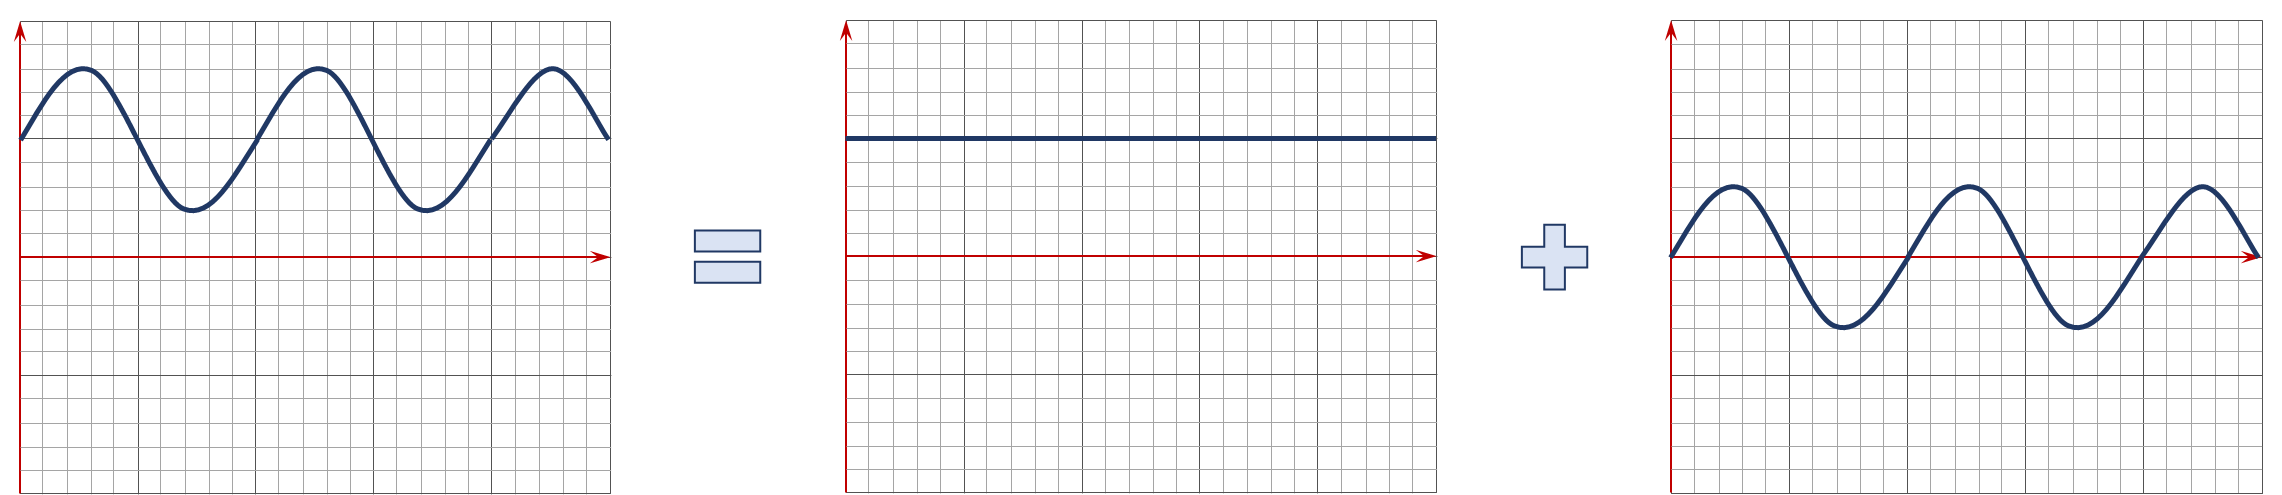
\includegraphics[width=\linewidth]{fig_04}
\caption{Décomposition d'un signal périodique\label{fig:ge:cours:04}}
\end{figure}

Sur les oscilloscopes : 
\begin{itemize}
\item en couplage DC le signal complet $s(t)$ est affiché;
\item en couplage AC seule la composante alternative $s_a(t)$ est affichée.
\end{itemize}

On a $\indice{S}{eff}^2 = \langle s \rangle^2 + \indice{S_a}{eff}^2$.

\subsection{Signal alternatif et sinusoïdal}

\begin{marginfigure}
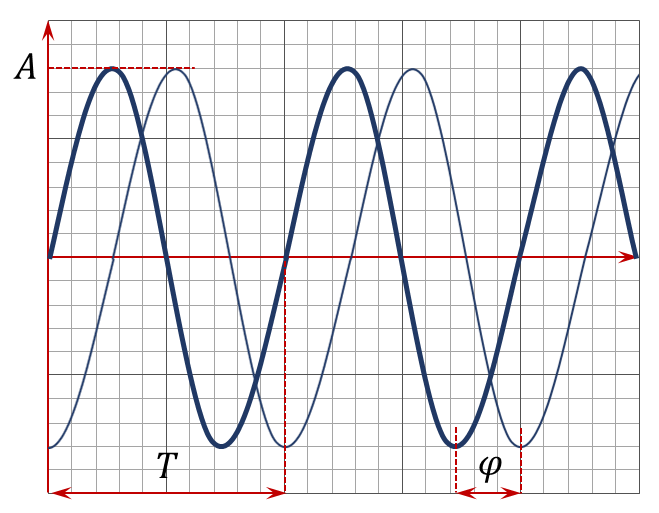
\includegraphics[width=\linewidth]{fig_05}
\caption{Signal alternatif sinusoïdal \label{fig:ge:cours:05}}
\end{marginfigure}
\begin{defi}
On note $s(t)=A\sin\left(\omega t + \varphi\right)$ avec : 
\begin{itemize}
\item  $A$ amplitude du signal;
\item  $\omega$ pulsation en $\si{rad.s^{-1}}$ tel que $\omega = 2\pi f = \dfrac{2\pi}{T}$;
\item  $\varphi$  déphasage.
\end{itemize}
\end{defi}


\begin{resultat}
Pour un signal sinusoïdal, on a $\indice{S}{eff}= \dfrac{A}{\sqrt{2}}$.
\end{resultat}
Pour un signal périodique, calculons la valeur efficace : 
$\indice{S}{eff} = \sqrt{\dfrac{1}{T} \int\limits_{0}^{T} A^2 \sin^2(\omega t + \varphi)\; \dd t}.$
$= \sqrt{\dfrac{ A^2}{2 T} \int\limits_{0}^{T} \left( 1 - \cos\left( 2\left(\omega t + \varphi\right)\right)\right)\; \dd t}$
$= \sqrt{\dfrac{ A^2}{2 T}\left( \left[t\right]_{0}^{T} -  \left[\dfrac{1}{2\omega}\sin\left( 2\left(\omega t + \varphi\right)\right)\right]_{0}^{T}  \right)}$

$= \sqrt{\dfrac{ A^2}{2 T}\left( T -  \dfrac{1}{2\omega}\left[
\sin\left( 2\left(\omega T + \varphi\right)\right)
- \sin\left( 2\left(\omega \times 0 + \varphi\right)\right)\right]  \right)}$
$= \sqrt{\dfrac{ A^2}{2 T}\left( T -  \dfrac{1}{2\omega}\left[
\sin\left( 2\left(\omega T + \varphi\right)\right)
- \sin\left( 2 \varphi\right)\right]  \right)}$. 
Avec $\varphi=0$, 
$\indice{S}{eff}= \sqrt{\dfrac{ A^2}{2 T}\left( T -  \dfrac{\sin\left( 2\omega T \right)}{2\omega}
  \right)}$
  $= \sqrt{\dfrac{ A^2}{2 T}\left( T -  \dfrac{\sin\left( 2\dfrac{2\pi}{T} T \right)}{2\dfrac{2\pi}{T}}  \right)}$
  $= \sqrt{\dfrac{ A^2}{2 T}T }$ $= \dfrac{A}{\sqrt{2}}$.


